\documentclass{optica-article}

\journal{opticajournal} % for journals or Optica Open

\articletype{Research Article}

\usepackage{lineno}
\linenumbers % Turn off line numbering for Optica Open preprint submissions.

\begin{document}

\title{Universal manuscript template for Optica Publishing Group journals}

\section{Abstract}
Lorem ipsum $\sim$ 100 words

\section{Introduction}
IR spectroscopy has seen significant interest and application in bio-imaging because it provides a chemical fingerprint of underlying samples in a label-free way \cite{baker_using_2014}. However, although the most relevant chemical information can be gathered in the mid-infrared ($\sim$ 3 - 12 $\mathrm{\mu m}$), slow signal acquisition is often a limiting factor, whose trade-off can keep it from competing with label-based fluorescence microscopy.

Fig.~\ref{fig:bckgnd} attempts to visualize the significant developments that have been made in mid-infrared hyperspectral imaging over roughly the last two decades. Experiments are mapped onto the two important metrics of spectra acquisition speed, which captures the rate at which spectra are gathered, and optical bandwidth, which captures the breadth of chemical content that can be observed. The two variables are plotted against each other, since a significant difficulty lies in achieving both metrics simultaneously. For a better one to one comparison, the acquisition speeds listed for experiments that use focal plane arrays have been normalized to that of an analogous point scanning experiment.

% why are these two important variables? Present it maybe as "information content"?

\begin{figure}[h]
    \centering
    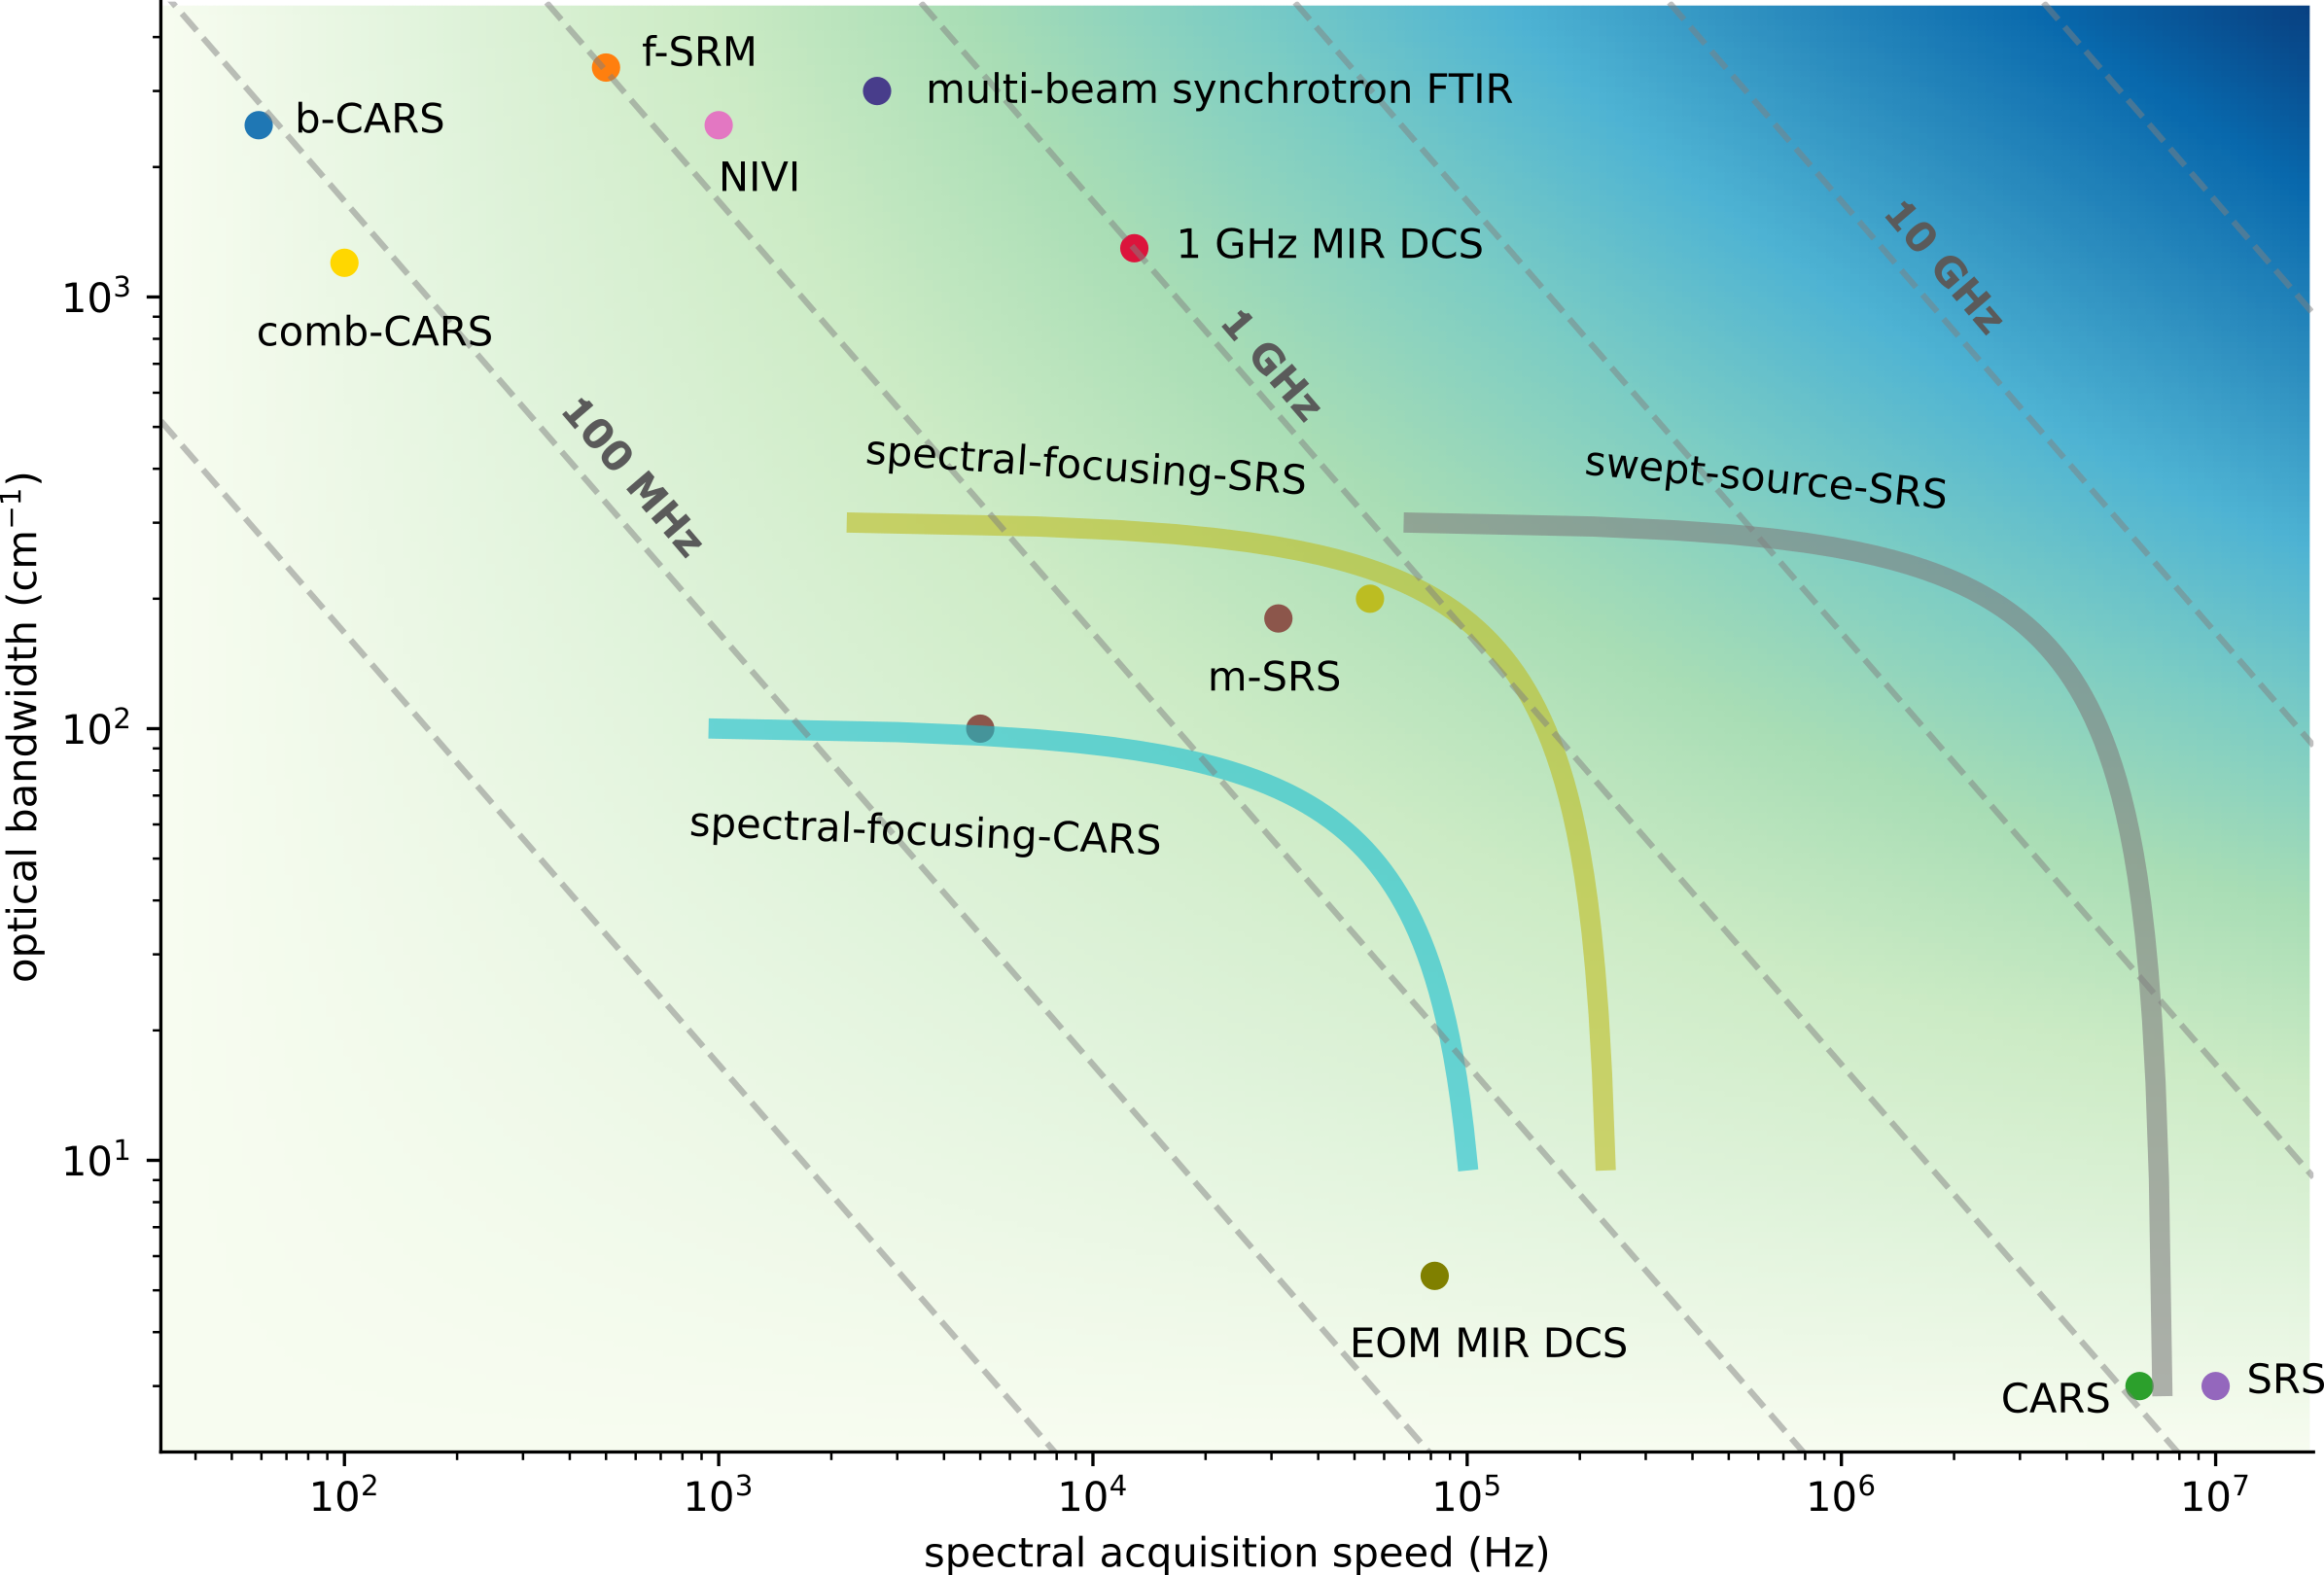
\includegraphics[width=\linewidth]{bckgnd_with_cm.png}
    \caption{Performance map of mid-infrared hyperspectral imaging. Broadband CARS (b-CARS) \cite{kee_simple_2004}, femtosecond Stimulated Raman Microscopy (f-SRM) \cite{ploetz_femtosecond_2007}, in-vivo video rate CARS \cite{evans_chemical_2005}, in-vivo video rate SRS \cite{saar_video-rate_2010}, multiplexed SRS (m-SRS) \cite{fu_quantitative_2012,liao_microsecond_2015}, nonlinear interferometric vibrational imaging (NIVI) \cite{chowdary_molecular_2010}, swept-source SRS \cite{ozeki_high-speed_2012}, spectral-focusing SRS \cite{fu_hyperspectral_2013}, spectral-focusing CARS \cite{di_napoli_hyperspectral_2014}, spectral-focusing SRS \cite{lin_microsecond_2021}, comb-CARS \cite{ideguchi_coherent_2013}, multi-beam synchrotron FTIR \cite{nasse_high-resolution_2011}, electro-optic modulator comb MIR DCS \cite{ullah_khan_direct_2020}}
    \label{fig:bckgnd}
\end{figure}

A few of the most notable experiments have utilized coherent Raman spectro-imaging, where in-vivo video-rate speeds have been demonstrated in the mid-infrared \cite{evans_chemical_2005, saar_video-rate_2010}. Whereas initial demonstrations were over a narrow bandwidth ($\sim$ 3  $\mathrm{cm^{-1}}$), broad bandwidths at high acquisition speeds have been demonstrated using rapidly rotating polygonal mirror scanners \cite{tamamitsu_ultrafast_2017, lin_microsecond_2021}. However, the stated metrics are only possible with the strong Raman absorption cross-sections around 2900~$\mathrm{cm^{-1}}$, which precludes Raman spectroscopy-based platforms from achieving the same performance in the fingerprint region at longer wavelengths.

Conversely, Fourier transform spectroscopy (FTS) and quantum cascade laser (QCL) based imaging are attractive due to their broad applicability across the mid to long wavelength infrared. The high absorption cross-sections can also alleviate the need for operation at powers close to sample-damage thresholds, a concern that is applicable to biological samples. In this category, FTS spectrometers coupled to broadband and bright sources such as synchrotron facilities have set the state of the art for the combination of spectral bandwidth and speed \cite{nasse_high-resolution_2011}. The coupling of broadband synchrotron light into a microscope requires the active stabilization of a beam bundle. However, a widely accessible imaging method would benefit from having a simple and table top setup. QCL lasers are attractive due to their direct emission in the mid-infrared and small footprint, although their performance is best leveraged in narrowband applications. Tunable QCL packages consisting of multiple QCL chips combined into one device \cite{yeh_fast_2015} can nominally reach broad spectral coverage, but struggle to reach noise figures comparable to platforms based on mode-locked lasers.

% need to address \cite{yeh_fast_2015}, which is a prime example of tunable QCL. The tunable QCL stuff is commercial, Rohith has one too. Why was he deprecating when it came to these? I recall it waas something about how the tuning is not so friendly as you would think. This is likely evidenced by the very noisy raw data they show in Fig. 2 of their paper. 
% The most recent Khan paper is a futher analysis of their previous work, particularly they go to very high frequency resolution which is a different direction than what you're discussing? They bring to light the QCL work though that I think we need to address ...

% something like: tunable QCL's consisting of multiple QCL chips can compensate the narrow spectral coverage, but without significant post-processing, so far struggle to reach noise figures comparable to light generated from mode-locked laser systems.

% version 2: tunable QCL's consisting of multiple QCL chips can nominally reach comparable spectral coverage, but in practice ... sounds too agressive.

More recently, dual-comb spectroscopy (DCS) in the frequency comb community has become a popular platform, due to its improved stability and speed when compared to classical FTS \cite{coddington_dual-comb_2016}. In this modality, the interference of two frequency combs maps a Nyquist band from the optical domain down into the RF. One of the most important considerations in DCS is the direct trade-off between the frequency resolution/repetition rate $f_r$ and the size of the optical Nyquist window $\Delta \nu$:
% 
\begin{align}
    \Delta \nu = \frac{f_r^2}{2 \Delta f_r}
\end{align}
% 
where $\Delta f_r$ is the interferogram acquisition rate equal to the difference of the two laser repetition rates. The diagonal dashed lines in Fig.~\ref{fig:bckgnd}., show the $f_r^2/2$ trade-off between resolvable bandwidth and acquisition speed in DCS for different repetition rates. Evidently, when broad absorption features allow for coarse resolution, the highest repetition rates are desired. However, in order to reach sufficient power per comb tooth, in practice the pulse energy required for nonlinear frequency down-conversion from the near-infrared sets an upper limit on the obtainable repetition rate. In this work, we utilize a set of recently developed 1-GHz mid-infrared frequency combs \cite{hoghooghi_broadband_2022} to integrate a dual-comb spectrometer with a confocal microscope. We capitalize on the high repetition rate by fully filling the third Nyquist band (2595$\mathrm{cm^{-1}}$--3890$\mathrm{cm^{-1}}$ at $\Delta f_r=12.86\text{kHz}$). The system is among the fastest performers in the class of spectrometers covering over 1000 $\mathrm{cm^{-1}}$ with high spectral resolution in the mid-infrared.

However, pointing to the dashed line in the upper right corner of Fig.~\ref{fig:bckgnd}, in order to achieve the ultimate goal of label-free broadband video-rate imaging, we note that the ideal DCS platform would operate with repetition rates of 10 GHz or higher. Such systems would likely require either high-power amplifiers or a nanophotonic design capable of generating equivalent bandwidths in the mid-infrared with pump pulse energies around 100 pJ.

% Compared to previous work in dual-comb MIR imaging \cite{ullah_khan_direct_2020}, we show

% compared to previous work in dual-comb mir imaging \cite{khan...}, we show a significant improvement over...
% actually not really a one to one comparison, just mention their work instead?

% in this work we use a recently developed 1 GHz ... coupled to a confocal microscope ... the pixels are scanned continusouly, the imaging speed is limited by the laser repetition rate of ... kHz

% The EOM MIR DCS is actually at 18 GHz, but they use an FPA so they can't go as fast as the repetition rate allows them for each pixel at a time.

\section{Experiment}

% you mentioned pulse energy difficulty before, maybe a brief but to the point statement of how this is achieved in this system

With long-term stability in mind, a single-branch intra-pulse difference frequency generation (DFG) design is used to generate light in the mid-infrared \cite{hoghooghi_broadband_2022}. 
% 
\begin{figure}[h]
    \centering
    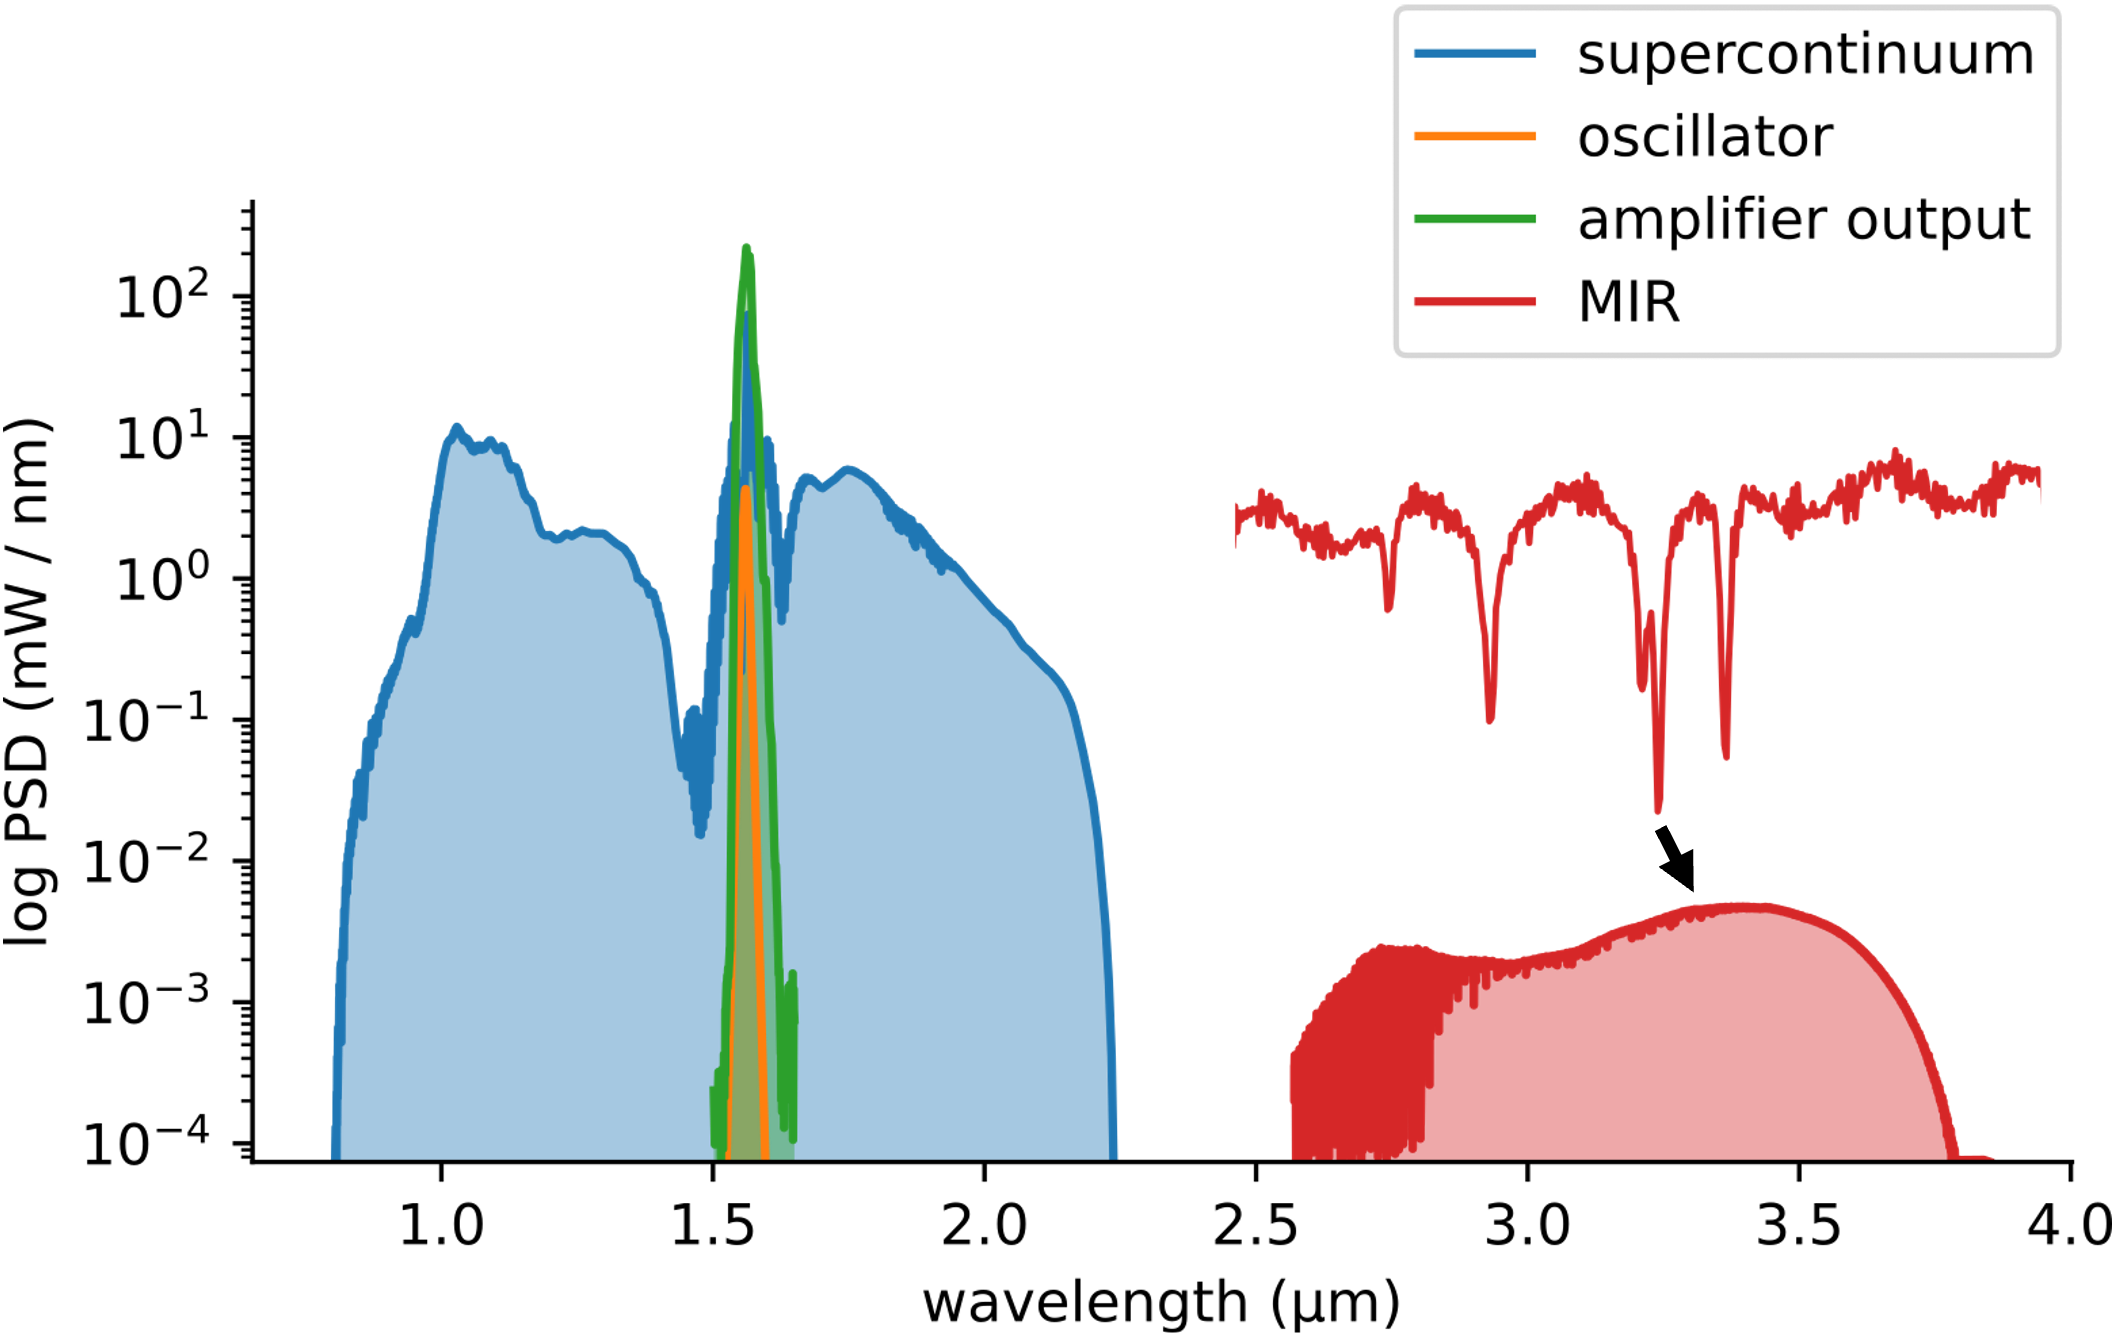
\includegraphics[width=\linewidth]{spectrum_in_setup.png}
    \caption{1 GHz MIR Frequency Comb. The spectral evolution through successive stages of the system: oscillator $\rightarrow$ chirped-pulse amplifier $\rightarrow$ few-cycle supercontinuum generation $\rightarrow$ MIR frequency down conversion. The inset shows a zoom in of waterlines that are resolved when using the full 1 GHz frequency resolution.}
    \label{fig:spectrum_in_setup}
\end{figure}
%
Shown in Fig. \ref{fig:spectrum_in_setup}, to compensate for the low conversion efficiency of the single-branch design, octave spanning few cycle NIR pulses generated via soliton self-compression in anomalous dispersion highly nonlinear fiber are used to drive the nonlinear frequency down conversion to the mid-infrared. Although coverage of the 6-12 $\mathrm{\mu m}$ wavelength region can be achieved for one laser system, due to the lack of nonlinear crystals in this work more widely available lithium niobate is used to cover the 3 - 5 $\mathrm{\mu m}$ wavelength window.

\begin{figure}[h]
    \centering
    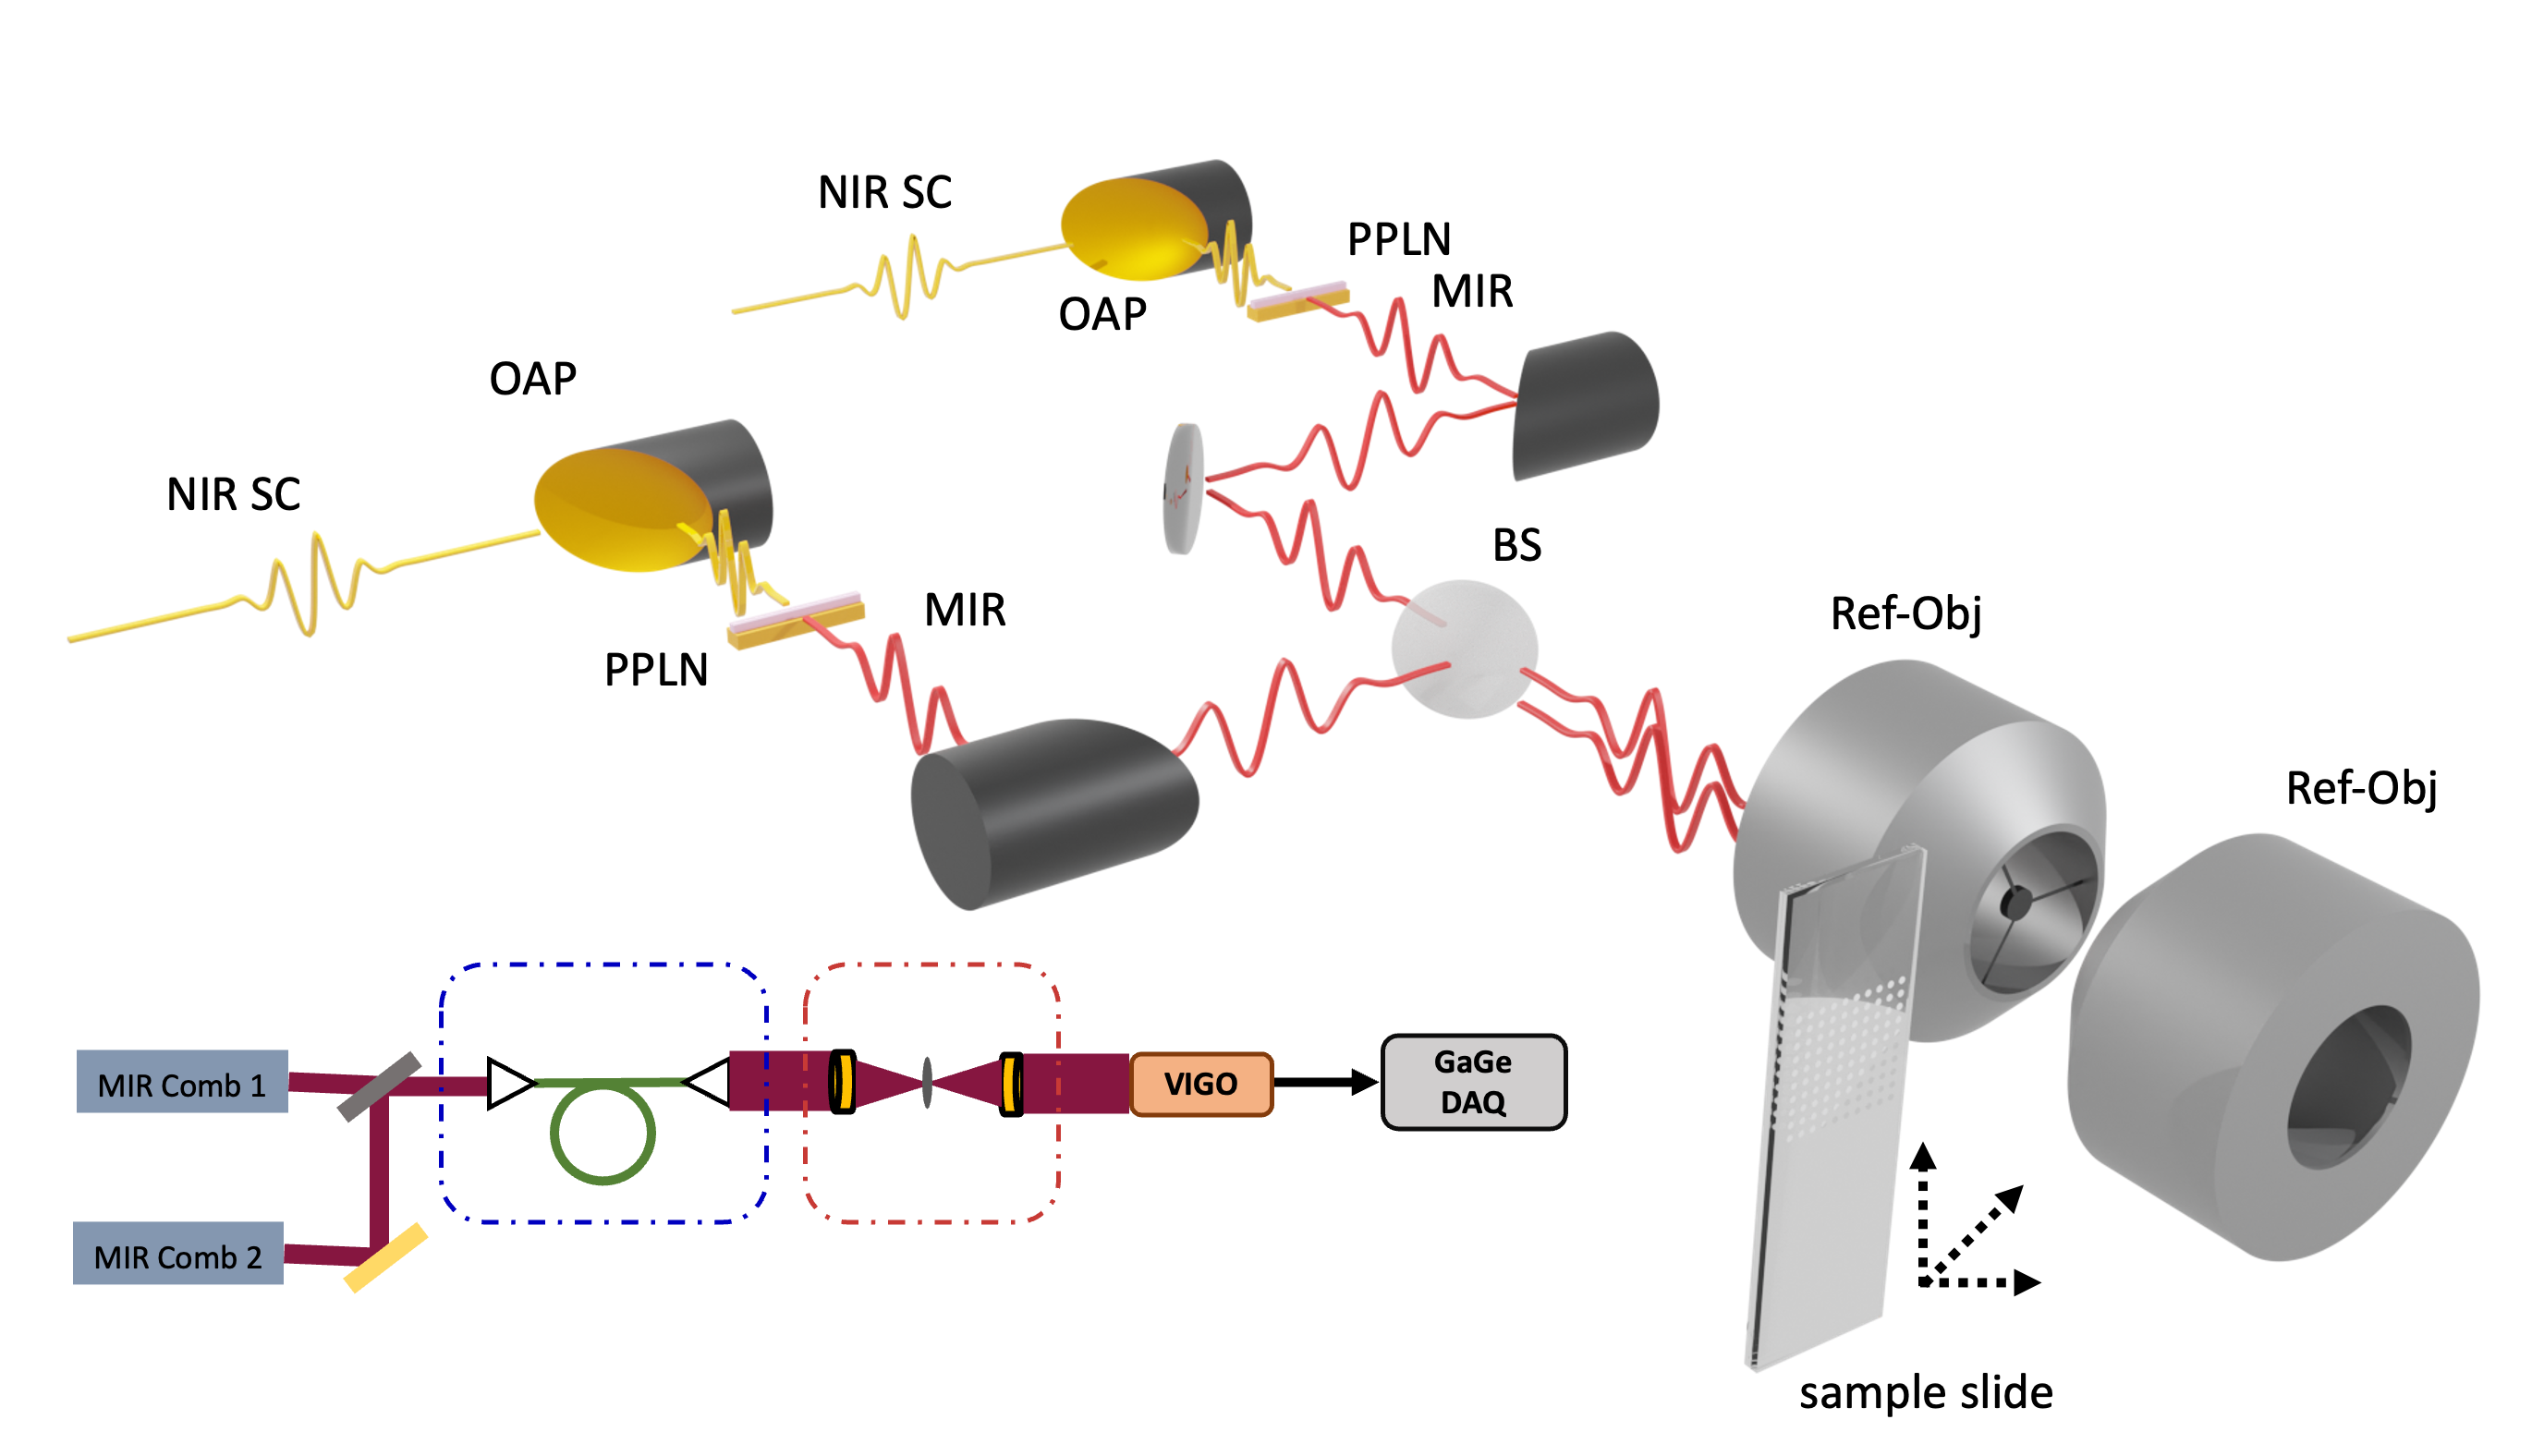
\includegraphics[width=\linewidth]{setup_3D.png}
    \caption{Experimental Setup. Two mid-infrared frequency combs generated through intra-pulse difference frequency generation are passed collinearly through a confocal microscope. Hyperspectral images are collected by raster scanning the sample slide. The transmitted signal is collected and digitized in a high-speed MCT mid-infrared detector and FPGA.}
    \label{fig:setup}
\end{figure}

Two 1-GHz mid-infrared frequency combs are generated and coupled into $\mathrm{InF_3}$ single-mode fiber for delivery to the experiment. The output beam is collimated with a two inch off-axis parabolic mirror, and a reflective confocal microscope with 0.58 NA is used to image the beam onto a glass slide ($\sim$~3.8 $\mathrm{\mu m}$ pixel size). A set of linear translation stages are used to raster scan the sample. The data is acquired via trigger, with the trigger spacing and scan speed set by the desired spatial sampling interval. The scan speed is limited by the interferogram acquisition time, which is fundamentally set by the repetition rate of the laser. The transmitted signal is focused onto a high-speed MCT detector, whose AC coupled port is digitized at 1 GS/s using an FPGA. The data is streamed concurrently from the card memory into PC RAM for real-time analysis, and such that the card-memory does not limit the data volume. Owing to the fairly high 500 MHz Nyquist frequency, and the placement of all fiber amplifiers in loop for the phase-locks of the two frequency combs, over one thousand interferograms can be directly averaged before phase correction needs to be employed.

\section{Results}

As a demonstration, hyperspectral images are taken of a USAF resolution target composed of SU-8 photoresist patterned onto a 500 $\mathrm{\mu m}$ thick Silicon wafer. Five hundred spectra are averaged at each pixel and apodized to 100 GHz (3.3 $\mathrm{cm^{-1}}$). The images are generated by integrating a 63$\mathrm{cm^{-1}}$ window around the peak absorption at 2930$\mathrm{cm^{-1}}$

using the peak absorbance value at The broad absorption of SU-8 is shown in Fig.~\ref{fig:su8}.~(b)., with the images 

\begin{figure}[h]
    \centering
    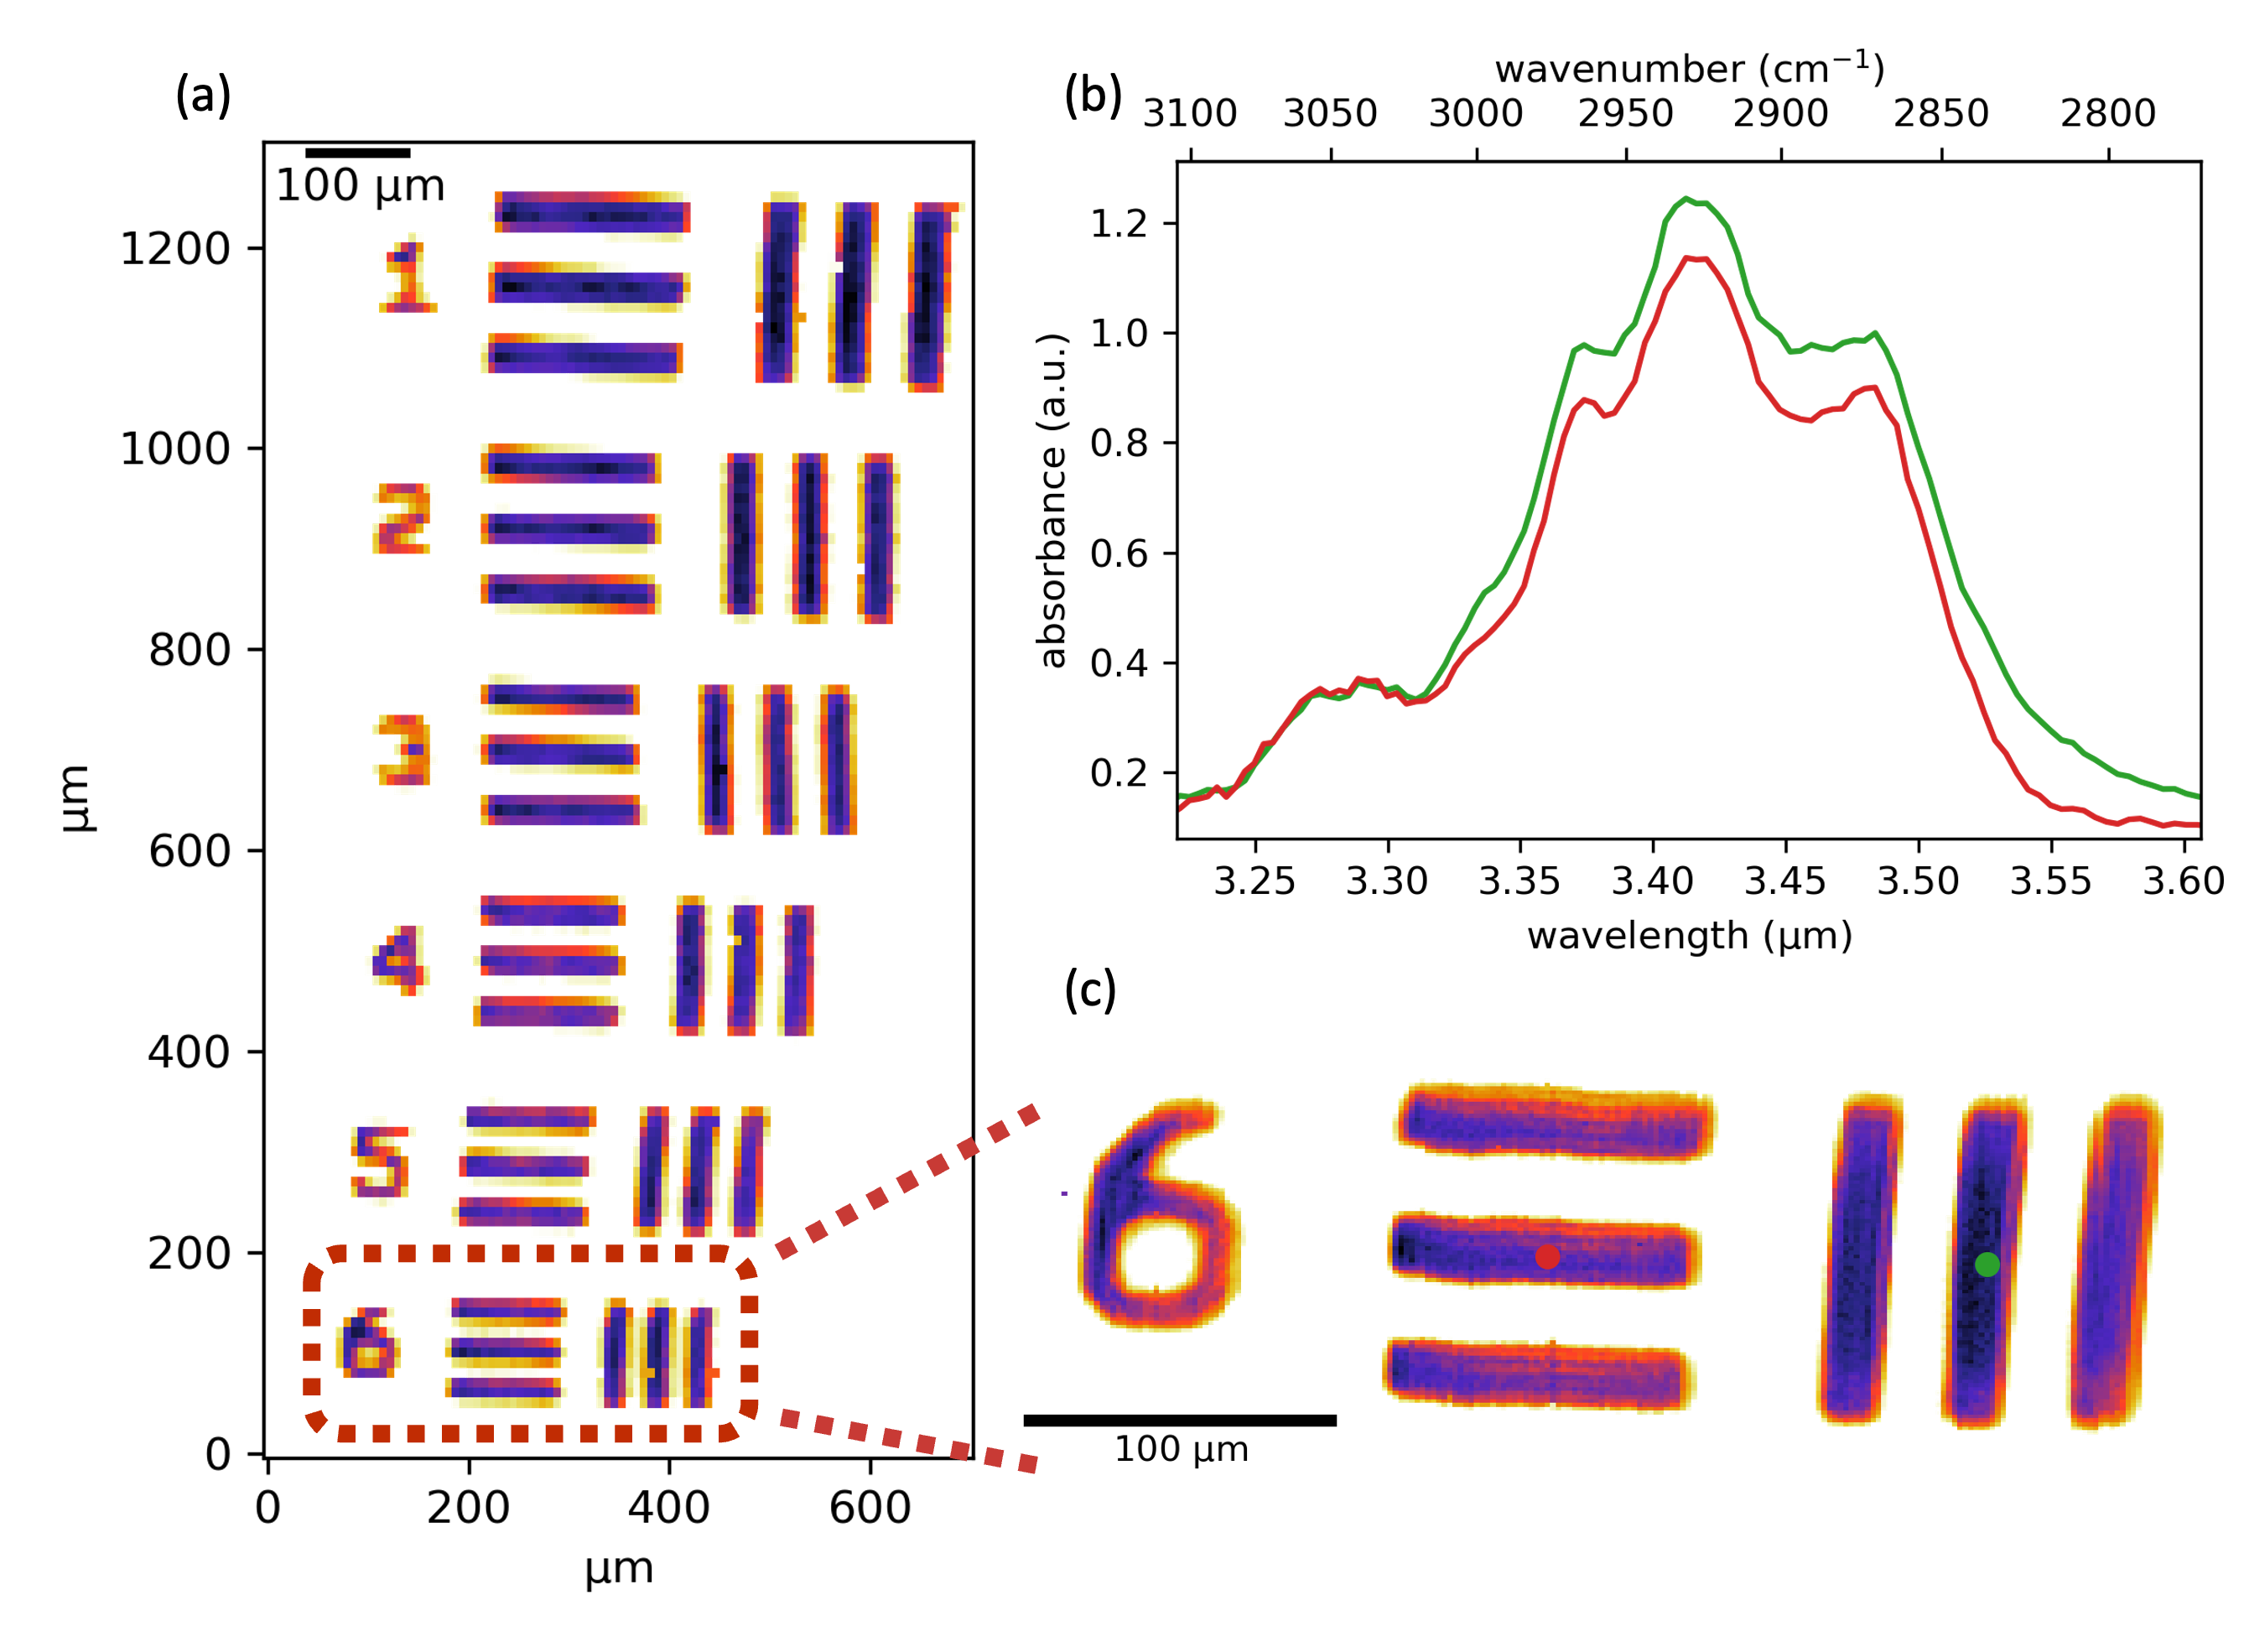
\includegraphics[width=\linewidth]{su8_image.png}
    \caption{Caption}
    \label{fig:su8}
\end{figure}

\begin{figure}[h]
    \centering
    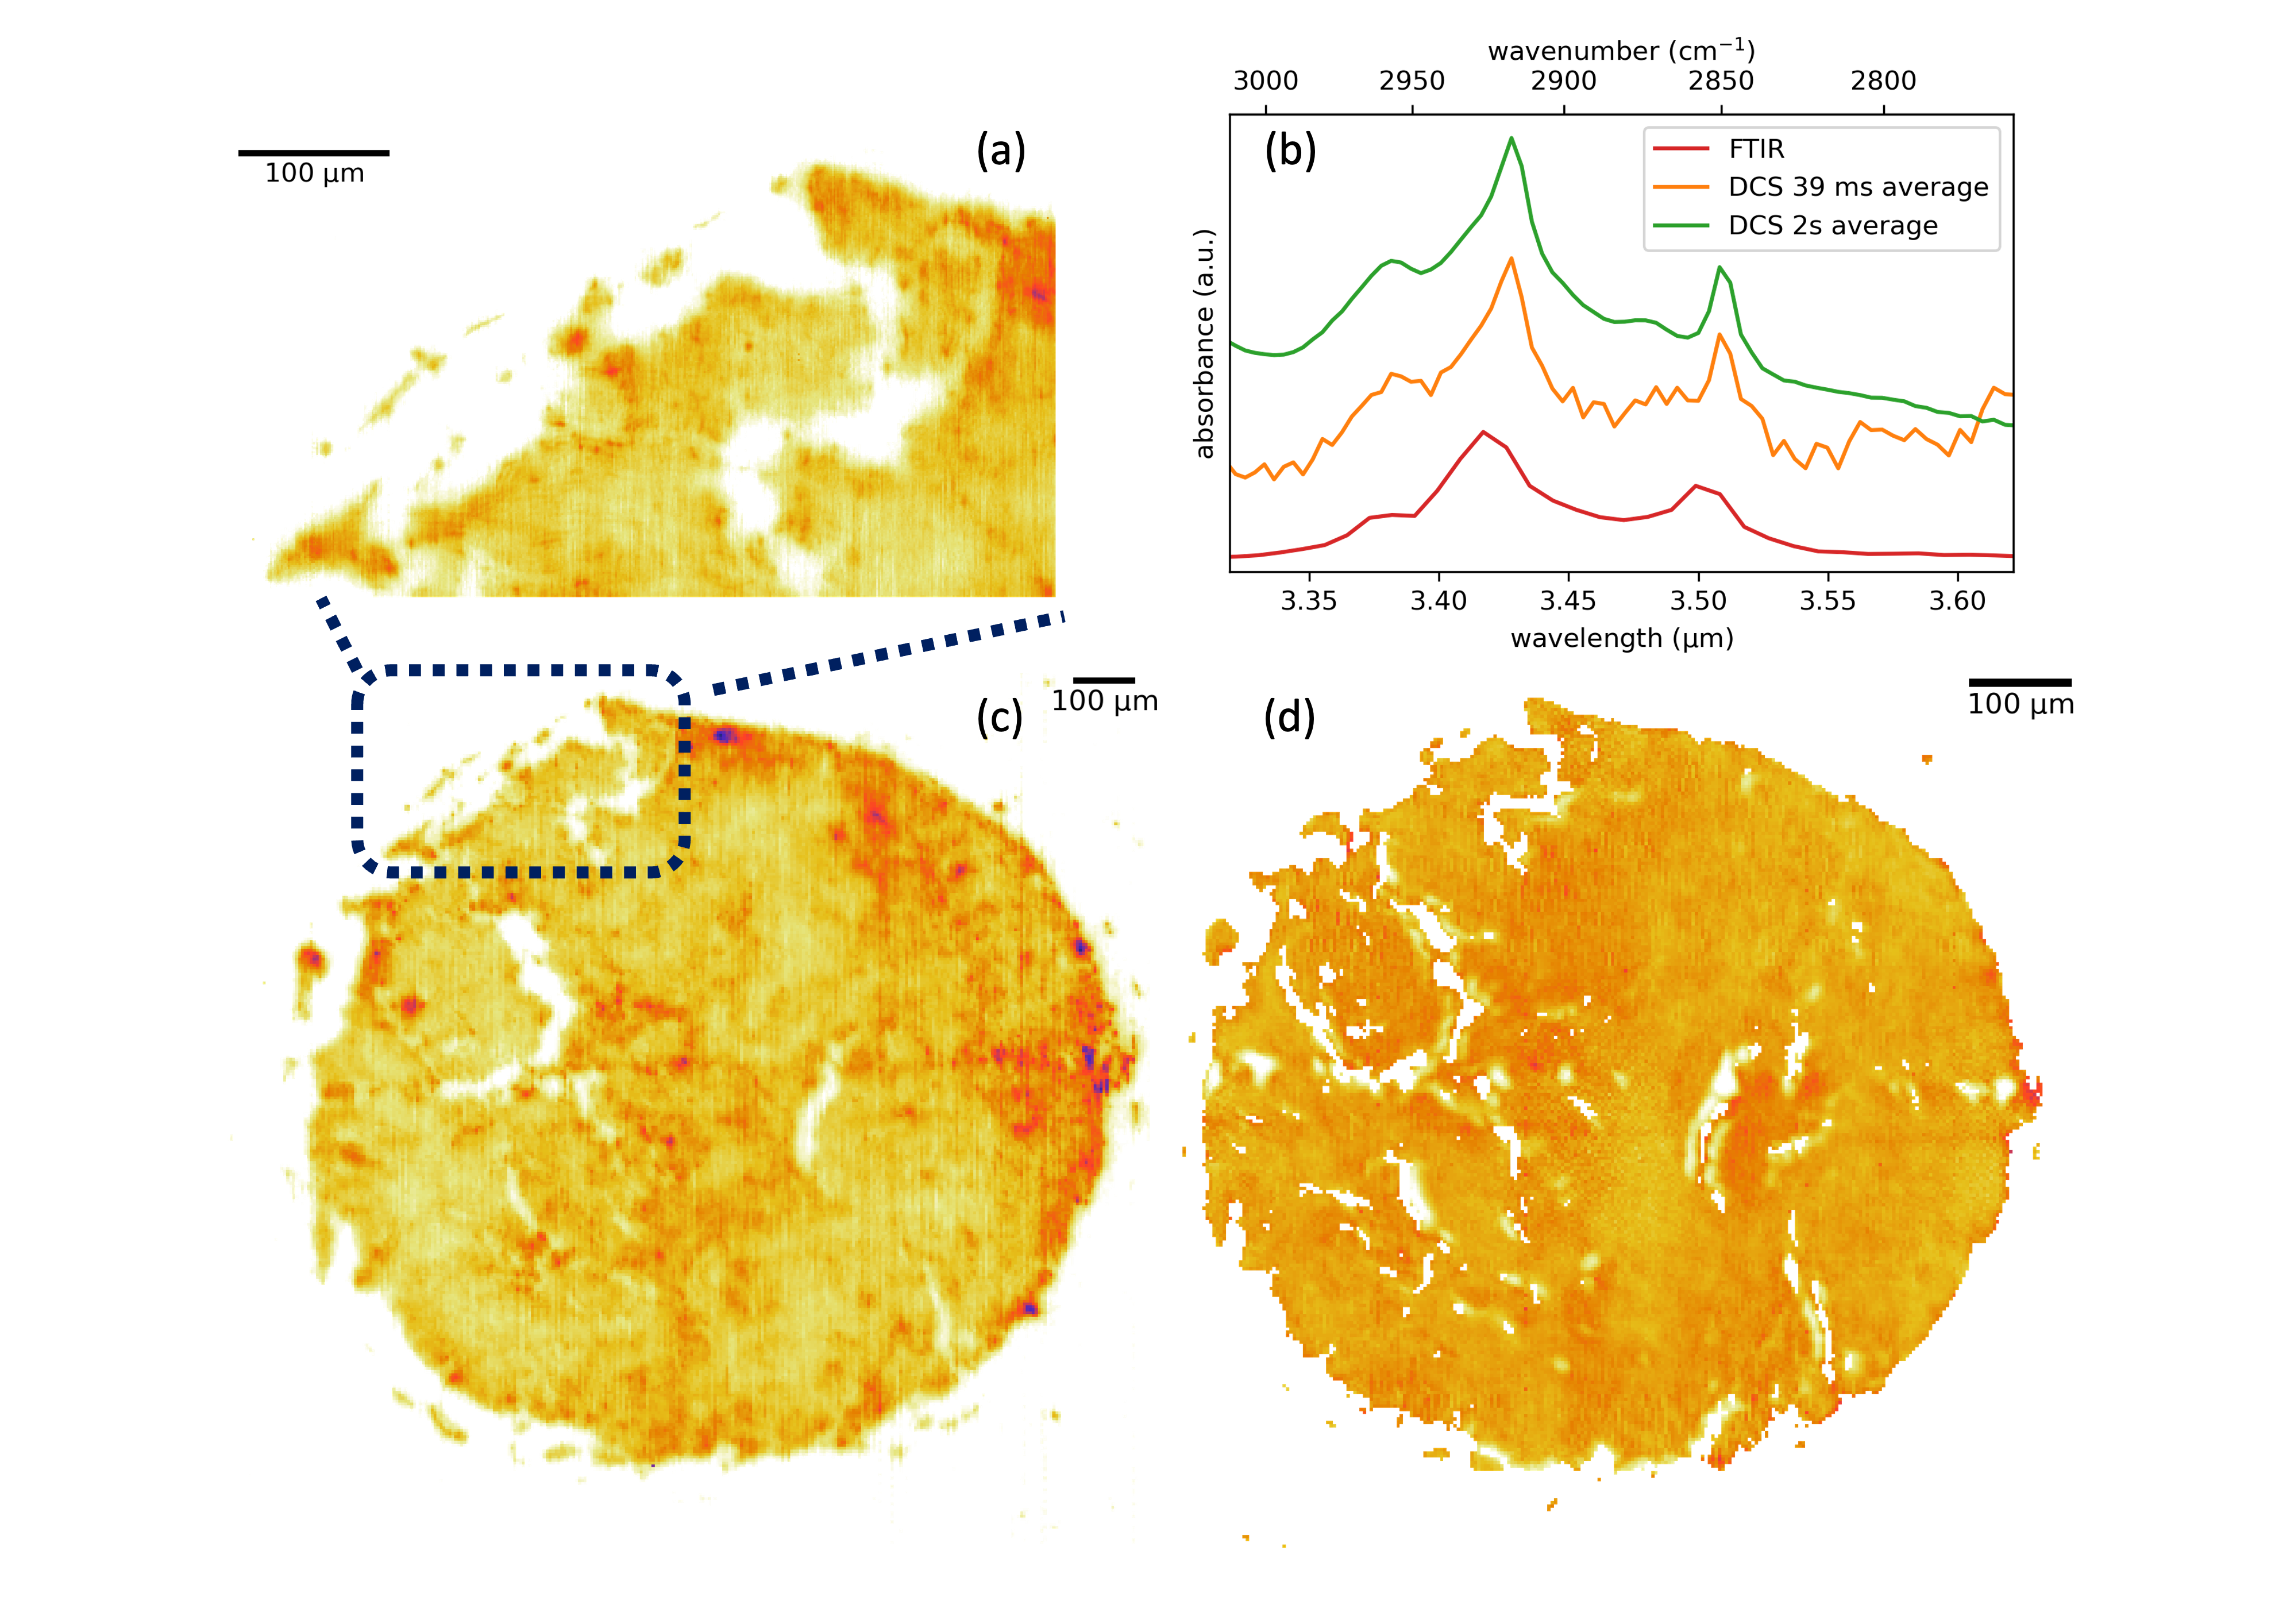
\includegraphics[width=\linewidth]{bio_image_w_FTIR_comparison.png}
    \caption{Caption}
    \label{fig:bio}
\end{figure}

\section{DCS Imaging Speed}
Regardless of the imaging method, the final determination of imaging speed is given by the time needed to reach sufficient SNR at each pixel. Specifically for DCS microscopy, the target SNR and frequency resolution sets the pixel dwell time. In DCS, the absorbance noise $\sigma$ scales with the frequency resolution and number of averaged spectra $N_{avg}$ according to \cite{newbury_sensitivity_2010}: 
% 
\begin{align}
    \sigma \propto \frac{N}{\sqrt{N_{avg}}}
    \label{eq:snr}
\end{align}
% 
where $N$ is the number of frequency bins. This scaling rule is shown in Fig.~\ref{fig:snr_analysis}.~(c-d)., where it is observed to match the experimentally measured absorbance noise. The two-variable map in  Fig.~\ref{fig:snr_analysis}.~(d). should apply more generally to to any DCS point scanning microscopy, but with the time axis scaled accordingly to the repetition rate. 

\begin{figure}[h]
    \centering
    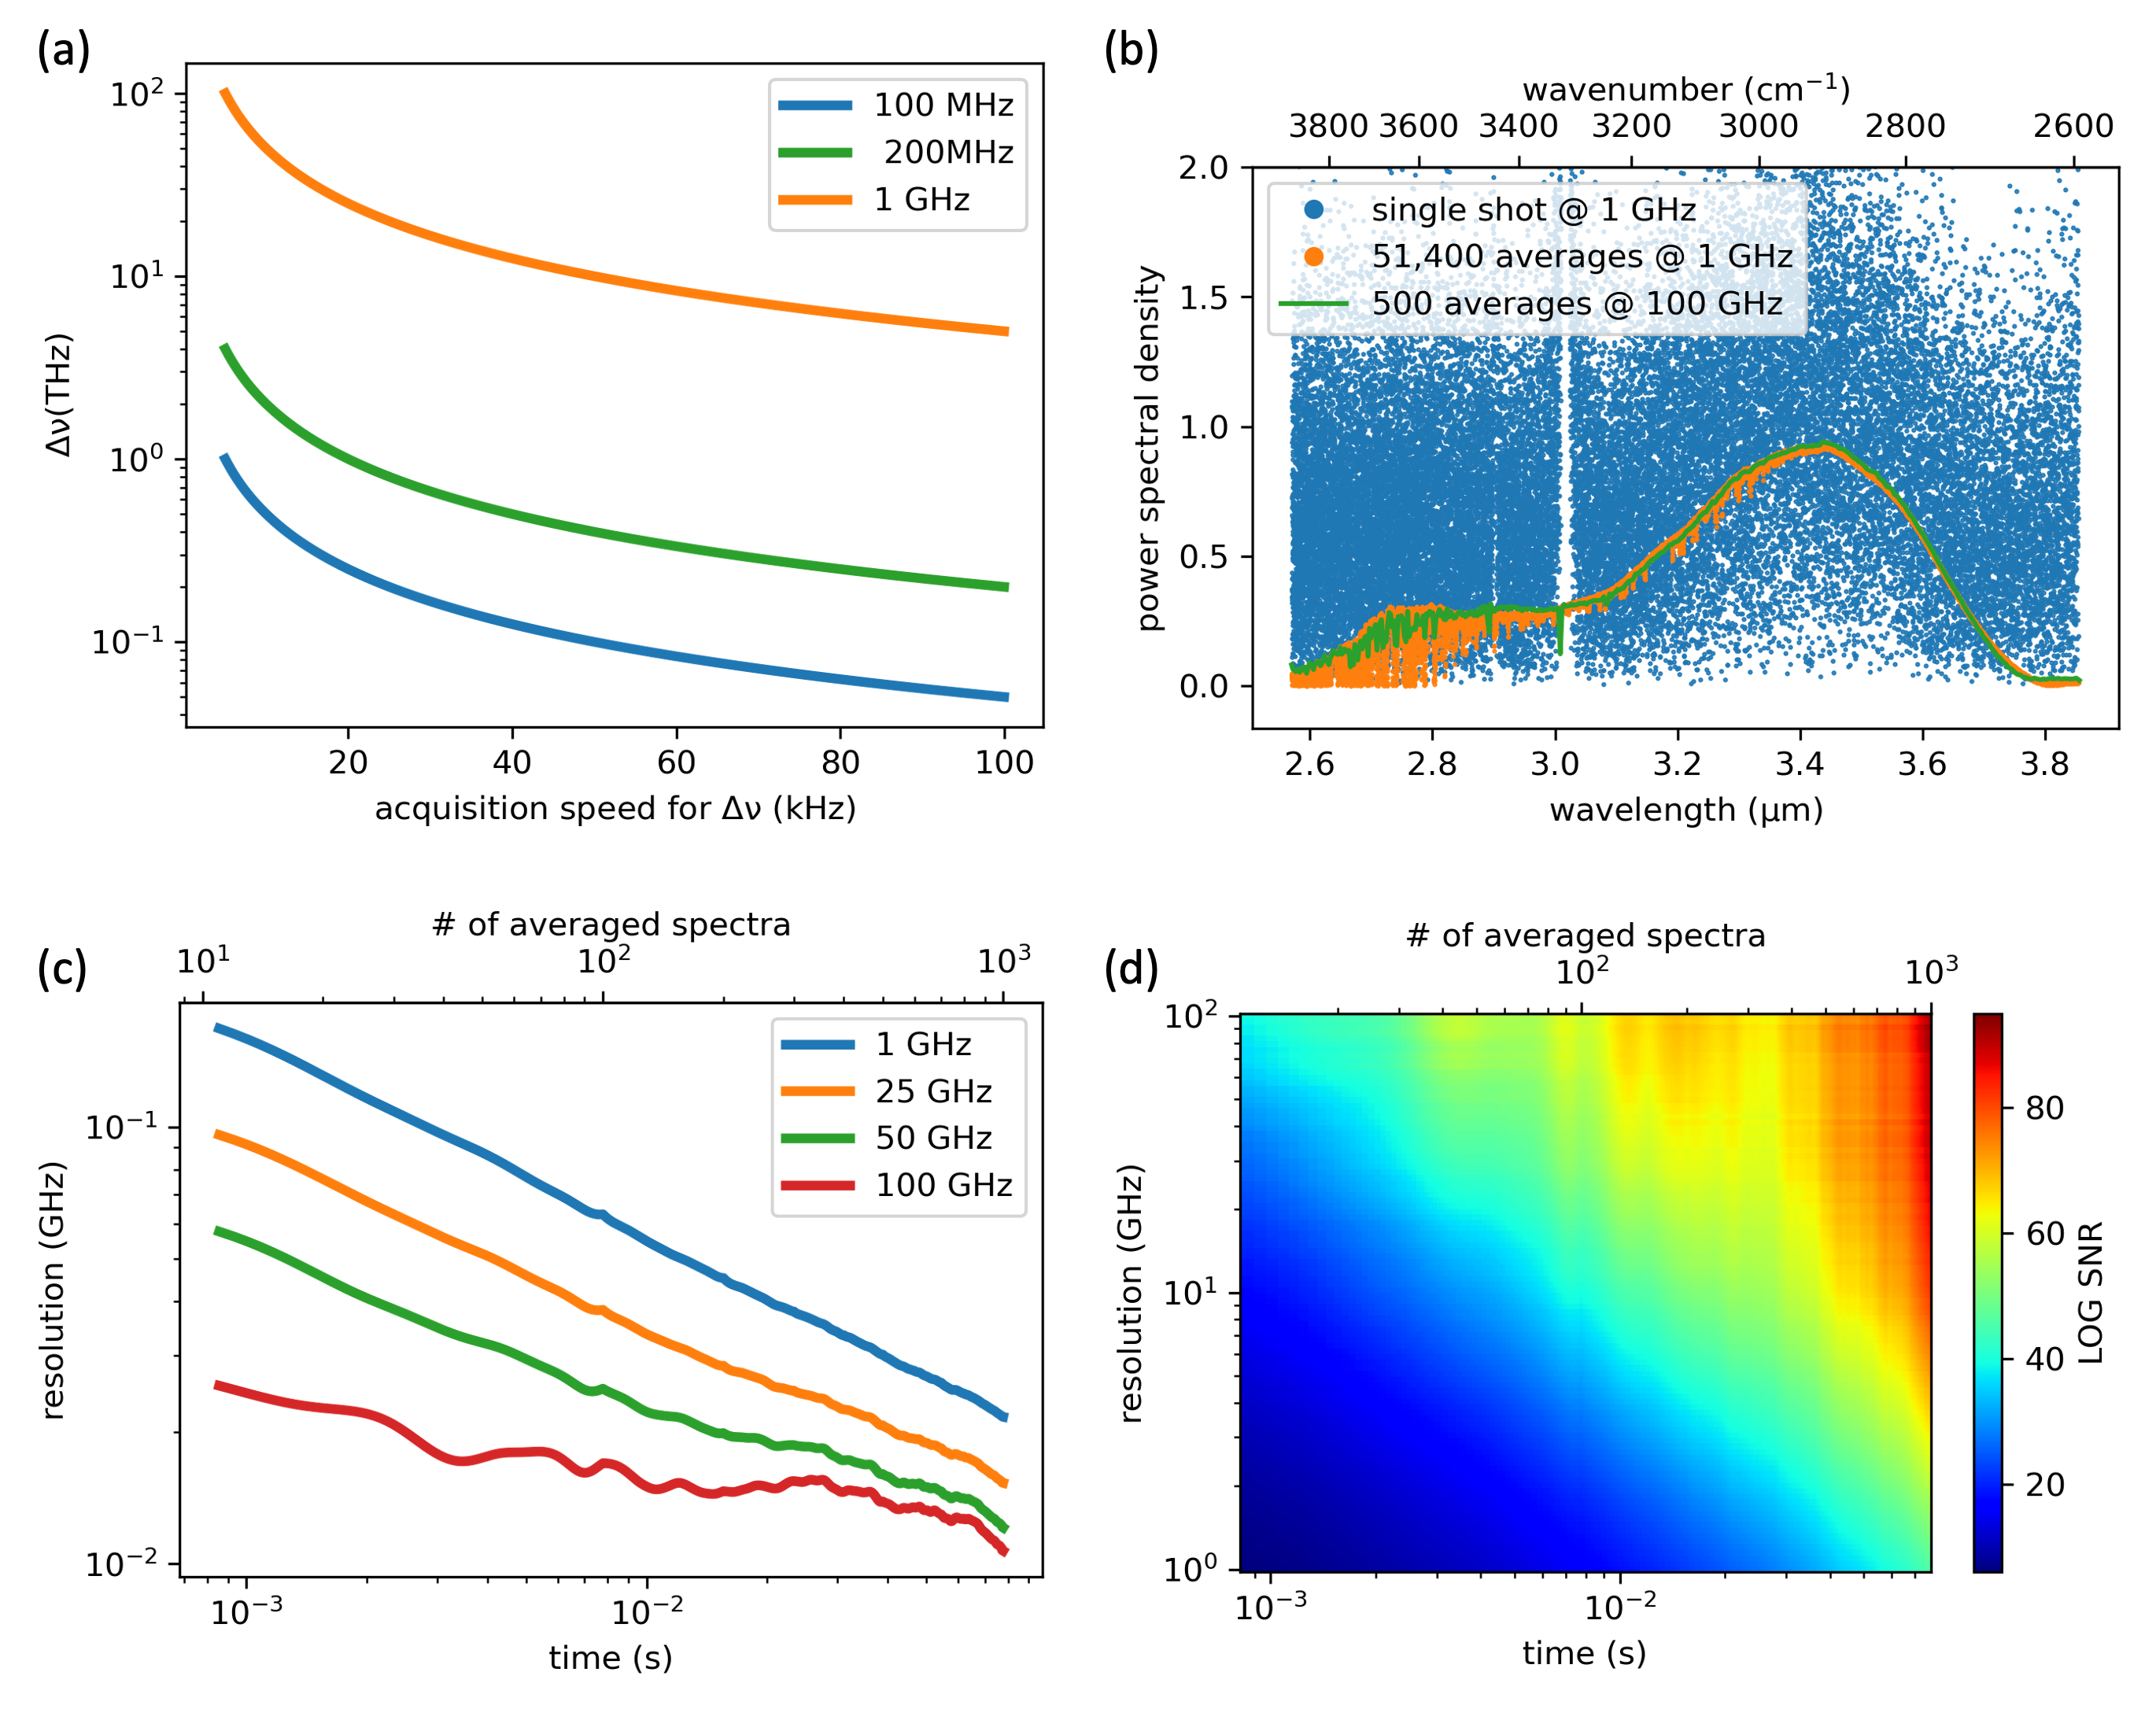
\includegraphics[width=\linewidth]{snr_analysis.png}
    \caption{Summary of DCS Imaging Speed. (a) The size of the optical Nyquist window plotted against acquisition speed ($\Delta f_r$) for different repetition rates. (b) DCS spectrum taken at different averaging times and frequency resolution/apodization windows. (c) The spectra's SNR follow the scaling of Eq.~\ref{eq:snr}, with an example of the 2D parameter space (d) mapped out for the 1-GHz system.}
    \label{fig:snr_analysis}
\end{figure}

Shown in Fig.~\ref{fig:snr_analysis}.~(a)., a baseline for 1 GHz DCS is that a 1000 $\mathrm{cm^{-1}}$ Nyquist window can be covered with $\sim$~17 kHz spectra acquisition speed, which is a two order magnitude improvement over well established 100 MHz mid-infrared dual-comb systems. In Fig.~\ref{fig:snr_analysis}.~(b)., a single-shot spectrum (77 $\mathrm{\mu s}$) at 1-GHz has low signal to noise, but can be averaged to high SNR in two seconds (>25,000 spectra). However, a high SNR can be achieved in $\sim$~39 ms at 500 averages if the interferograms are apodized to 100 GHz ($\sim$~3.33 $\mathrm{cm^{-1}}$).  The SNR as a function of averaging time and frequency resolution is shown in Fig.~\ref{fig:snr_analysis}.~(c-d).; the absorbance noise always averages down according to $1/\sqrt{N_{avg}}$, but with coarser resolution resulting in a directly proportional overall noise reduction. 

% it's important to note, that all this analysis concerns data prior to any additional SNR enhancement via post-processing. So, it does not preclude those methods. But adding that dimension should just mean you can live with acquiring less SNR and move all the curves down by whatever factor the post-processing buys you in terms of SNR. I think this is especially relevant for the QCL stuff

% merge conflict example
here is a merge conflict: HELLO WORLD

\bibliography{references}

\end{document}
